\documentclass[a4paper,12pt]{article}

\usepackage[english]{babel}
\usepackage[T1]{fontenc}
\usepackage[utf8]{inputenc}
\usepackage{amsmath}
\usepackage{amsthm}
\usepackage{graphicx}

\usepackage{geometry}
\geometry{total={210mm,297mm},
left=20mm, right=20mm,
bindingoffset=0mm,
top=20mm, bottom=20mm}

\usepackage[
  pdftitle={Homework 2},
  pdfauthor={William Jagels},
  colorlinks=true,linkcolor=blue,urlcolor=blue,citecolor=blue,bookmarks=true,
bookmarksopenlevel=2]{hyperref}

\usepackage{titlesec}
\titlelabel{\thetitle.\quad}

\def\code#1{\texttt{#1}}

\title{Homework 2}

\author{William Jagels}

\date{\today}

\begin{document}
\maketitle

\section{}
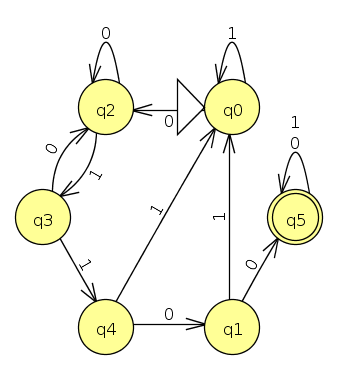
\includegraphics[width=15cm]{question1}

\section{}
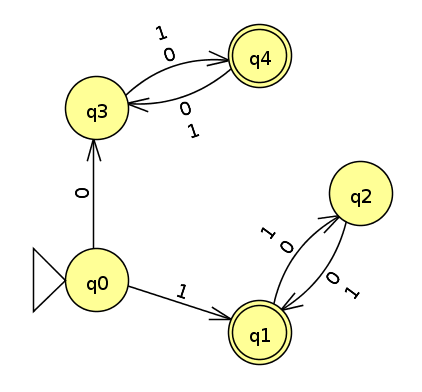
\includegraphics[width=15cm]{question2}
\section{}
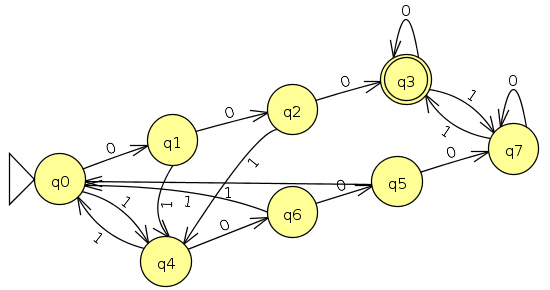
\includegraphics[width=15cm]{question3}
\section{}
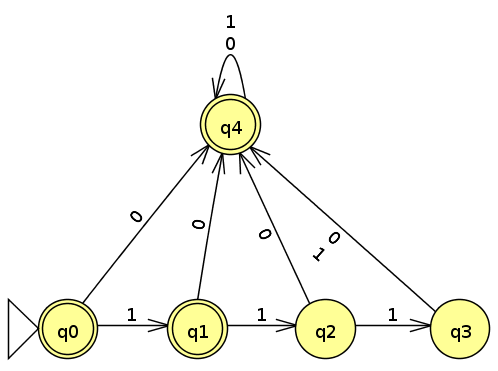
\includegraphics[width=15cm]{question4}
\section{}
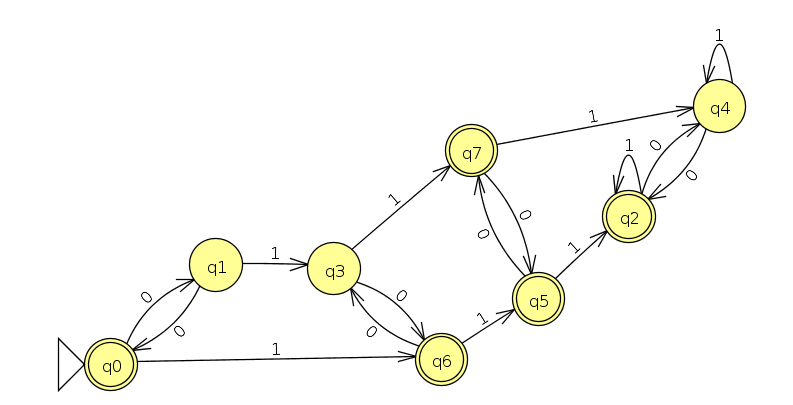
\includegraphics[width=15cm]{question5}
\section{}
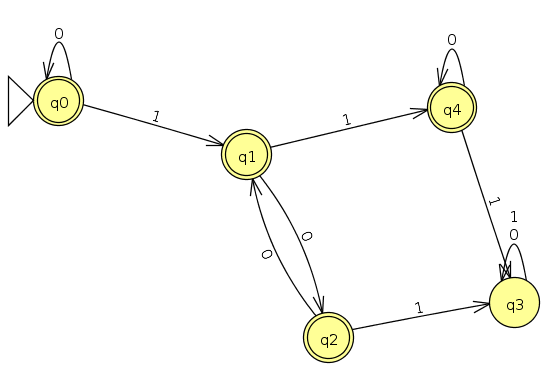
\includegraphics[width=15cm]{question6}
\section{}
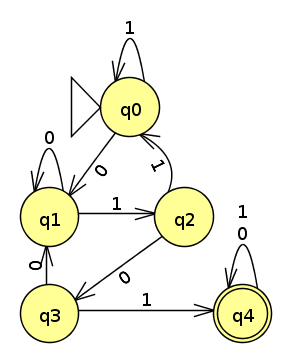
\includegraphics[width=15cm]{question7}
\section{}
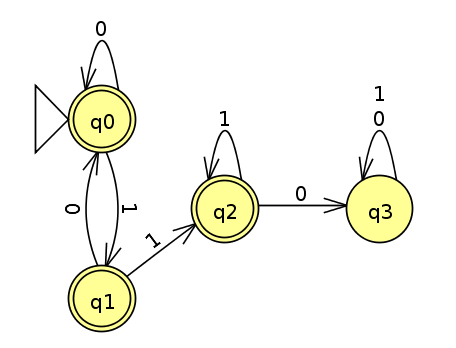
\includegraphics[width=15cm]{question8}

\section{}
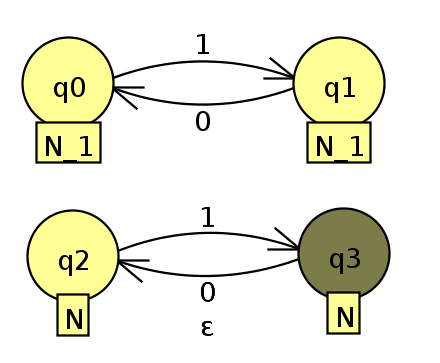
\includegraphics[width=15cm]{question9}

\section{}
If you craft some NFA that recognizes the input string.
Then flip all the arrows, and use the start state as the one accept state.
For the start state, create a new one and connect it to the old accept
states with $\epsilon$-transitions.
Since an NFA recognizes the language, it is regular.

\end{document}
